\documentclass{article}
\usepackage{verbatim}
\usepackage{fullpage}
\usepackage{amsmath}
\usepackage{graphicx}
\usepackage{listings}
\usepackage{placeins} % for \FloatBarrier
%% package for contiued float
\usepackage{caption}
\usepackage[english,greek, main=greek]{babel}
\usepackage[utf8]{inputenc}
\useshorthands{;}
\defineshorthand{;}{?}

\usepackage{pythonhighlight}

\usepackage[explicit]{titlesec} % number after section name
%% the following lines are used to reset the section counter
%% after 'part' is encountered.
\makeatletter
\@addtoreset{section}{part}
\makeatother
%% the following lines are used to add the section number
%% after the section name
\titleformat{\section}
  {\normalfont\large\bfseries}
  {}
  {0em}
  {#1\ \thesection}
%% number after subsection name
\titleformat{\subsection}
  {\normalfont\large\bfseries}
  {}
  {0em}
  {#1\ \thesubsection}
%% avoid numbering contents
\titleformat{\section}
  {\normalfont\Large\bfseries}
  {}
  {0em}
  {\ifnum\value{section}=0\relax #1\else #1\ \thesection\fi}
\newcommand{\eng}[1]{\foreignlanguage{english}{#1}} % shortcut for inserting english into greek text


\title{
    \includegraphics[width=\textwidth]{~/Pictures/emp.png} \\
    \vskip 5cm
    Νευροασαφής Έλεγχος και Εφαρμογές\\
    \large Άσκηση 3η
    \vskip 5cm
}

\author{Αναστάσιος Στέφανος Αναγνώστου\\
        03119051}

\begin{document}

\maketitle
\newpage
\tableofcontents
\newpage

\part{Αλγόριθμοι Βελτιστοποίησης}

Αρχικά, για όλες τις ασκήσεις του μέρους αυτούς, γράφηκαν κατάλληλες
συναρτήσεις που υλοποιούν τους διαφόρους αλγορίθμους βελτιστοποίησης.
Παρατίθενται όλες εδώ:

\selectlanguage{english}
\begin{python}
import numpy as np 

def gradient_descent(f, df, x_curr, a, eps=0.001, limit=1000):
    value = f(*x_curr)
    delta = df(*x_curr)
    x_next = x_curr - a * delta 
    nvalue = f(*x_next)
    iterations = 0
    while abs(value - nvalue) > eps and iterations < limit:
        value = nvalue
        delta = df(*x_next)
        x_next = x_next - a * delta 
        nvalue = f(*x_next)
        iterations += 1
    return nvalue, x_next, iterations

def newtons_method(f, df, ddf, x_curr, a, eps=0.001, limit=1000):
    x_next = x_curr - df(*x_curr) / ddf(*x_curr)
    value = f(*x_curr)
    nvalue = f(*x_next)
    iterations = 0
    while abs(value - nvalue) > eps and iterations < limit:
        value = nvalue
        x_next += -df(*x_next) / ddf(*x_next)
        nvalue = f(*x_next)
        iterations += 1
    return nvalue, x_next, iterations

def momentum_method(f, df, x_curr, a1, a2, eps=0.001, limit=1000):
    v_curr = np.array([0, 0])
    v_next = a1 * v_curr - a2 * df(*x_curr)
    x_next = x_curr + v_next
    iterations = 0;
    while abs(f(*x_curr) - f(*x_next)) > eps and iterations < limit:
        v_curr = v_next
        x_curr = x_next
        v_next = a1 * v_curr - a2 * df(*x_curr)
        x_next = x_curr + v_next
        iterations += 1;
    return f(*x_next), x_next, iterations
\end{python}
\selectlanguage{greek}

\clearpage
\section{Θέμα}

Εξετάζεται η σύγκλιση του αλγορίθμου \eng{gradient descent} για την εύρεση του
ελαχίστου της συνάρτησης $f(x_1,x_2) = x_1^2 +(x_2 - 1)^2 + (x_1 - x_2)^4$, για
τα διάφορα μεγέθη βήματος.

\selectlanguage{english}
\begin{python}
def f(x1, x2):
    return x1**2 + (x2 - 1)**2 + (x1 - x2)**4

def df(x1, x2):
    return np.array([2*x1 + 4*(x1 - x2)**3, 2 *(x2 - 1) - 4*(x1 - x2)**3])

def ddf(x1, x2):
    return (4 + 24*(x1 - x2)**2)

if __name__ == '__main__':
    np.set_printoptions(precision=3)
    steps = [0.1 - 0.01 * i for i in range(0, 10)]
    initial = np.array([2, 5])
    for step in steps:
        minimum, minimizer, loops = gradient_descent(f, df, initial, step)
    steps = [0.1 + 0.1 * i for i in range(0, 10)]
    for step in steps:
        minimum, minimizer, loops = newtons_method(f, df, ddf, initial, step)
\end{python}
\selectlanguage{greek}

\clearpage
\section{Θέμα}

Για τον υπολογισμό του \eng{condition number} της παράστασης $f(x1, x2) = A
\cdot x_1^2 + \frac{1}{A} \cdot x_2^2$, γράφτηκε ο παρακάτω κώδικας σε
\eng{Python}.

\selectlanguage{english}
\begin{python}
def f(x1, x2, A=10):
    return A*x1**2 + (1/A)*x2**2
def df(x1, x2, A=10):
    return np.array([2*A*x1, (2/A)*x2])
def ddf(x1, x2, A=10): # not actually a function of x1, x2
    return 2*A + (2/A)
if __name__ == '__main__':
    As = [1.2*i for i in range(1, 11)]
    initial = np.array([50, -100]) # initial guess for the minimizer
    for A in As:
        min, minimizer, loops = gradient_descent(lambda x1, x2: f(x1, x2, A),
                                                 lambda x1, x2: df(x1, x2, A),
                                                 initial, 0.05)
        cond = max(2*A, 2/A)/min(2*A, 2/A) # condition number of hessian
    for A in As:
        min, minimizer, loops = momentum_method(lambda x1, x2: f(x1, x2, A),
                                                lambda x1, x2: df(x1, x2, A),
                                                initial, 0.5, 0.05)
        cond = max(2*A, 2/A)/min(2*A, 2/A)
\end{python}
\selectlanguage{greek}

Παρατίθενται τα αποτελέσματα των δύο αλγορίθμων βελτιστοποίησης για τις
διάφορες τιμές του Α. Σε κάθε γραμμή φαίνεται το Α, το \eng{condition number},
η ελάχιστη τιμή, το σημείο ελαχιστοποίησης και ο αριθμός των επαναλήψεων.

\selectlanguage{english}
\begin{verbatim}
========= ========= gradient descent ========= =========
A = 1.200, Cond num = 1.440: 0.004, [ 0.001 -0.073], 82
A = 2.400, Cond num = 5.760: 0.011, [ 5.033e-17 -1.618e-01], 150
A = 3.600, Cond num = 12.960: 0.017, [ 2.602e-40 -2.478e-01], 212
A = 4.800, Cond num = 23.040: 0.023, [ 5.443e-76 -3.328e-01], 270
A = 6.000, Cond num = 36.000: 0.029, [ 9.344e-129 -4.173e-001], 325
A = 7.200, Cond num = 51.840: 0.035, [ 1.485e-208 -4.988e-001], 378
A = 8.400, Cond num = 70.560: 0.041, [ 0.    -0.587], 428
A = 9.600, Cond num = 92.160: 0.047, [ 0.   -0.67], 477
A = 10.800, Cond num = 116.640: 0.053, [ 0.    -0.757], 524
A = 12.000, Cond num = 144.000: 0.059, [ 0.    -0.841], 570
\end{verbatim}
\selectlanguage{greek}

Κάτι που παρατηρείται είναι ότι όσο αυξάνεται το \eng{condition number} του
πίνακα \eng{Hessian} τόσο αυξάνεται και ο αριθμός των επαναλήψεων που
απαιτούνται για την σύγκλιση του αλγορίθμου \eng{gradient descent}.

\selectlanguage{english}
\begin{verbatim}
========= ========= momentum method  ========= =========
A = 1.200, Cond num = 1.440: 0.001, [ 0.001 -0.03 ], 31
A = 2.400, Cond num = 5.760: 0.004, [-4.210e-10 -1.028e-01], 71
A = 3.600, Cond num = 12.960: 0.008, [-3.105e-15 -1.653e-01], 105
A = 4.800, Cond num = 23.040: 0.010, [ 2.768e-20 -2.222e-01], 137
A = 6.000, Cond num = 36.000: 0.013, [-2.347e-24 -2.819e-01], 167
A = 7.200, Cond num = 51.840: 0.016, [ 1.103e-28 -3.383e-01], 196
A = 8.400, Cond num = 70.560: 0.019, [-1.113e-33 -4.040e-01], 223
A = 9.600, Cond num = 92.160: 0.022, [ 5.048e-37 -4.607e-01], 250
A = 10.800, Cond num = 116.640: 0.025, [ 1.095e-40 -5.195e-01], 276
A = 12.000, Cond num = 144.000: 0.028, [-6.123e-45 -5.813e-01], 301
\end{verbatim}
\selectlanguage{greek}

Φαίνεται ότι ο αλγόριθμος \eng{momentum method} είναι πιο αποδοτικός από τον
αλγόριθμο \eng{gradient descent}. Αν και για μικρά \eng{condition numbers} οι
δύο αλγόριθμοι βρίσκουν κοντινά ελάχιστα, όσο αυτοί αυξάνονται ο αλγόριθμος
\eng{gradient descent} αρχίζει να αποκλίνει από την ελάχιστη τιμή.
Ο δε αλγόριθμος \eng{momentum method} παραμένει σταθερός και βρίσκει την
ελάχιστη τιμή, μάλιστα σε μικρότερο αριθμό επαναλήψεων.

\clearpage
\section{Θέμα}

Εξετάζεται ο \eng{condition number} του πίνακα $Q = A \cdot A^T$ όπου $A$ είναι
τυχαίος πίνακας, σαν συνάρτηση της διάστασης του $A$. Για κάθε διάσταση
παράγεται ένας αριθμός τυχαίων πινάκων και υπολογίζεται ο μέσος όρος των
\eng{condition numbers}. Ο μέσος όρος μπορεί να υπολογιστεί με πολλούς τρόπους,
παραδείγματος χάριν, ως αριθμητικός μέσος όρος ή ως αρμονικός μέσος όρος. Ο
κώδικας επιδεικνύει τον υπολογισμό του αριθμητικού μέσου όρου, όμως στα
αποτελέσματα παρουσιάζονται περισσότεροι.

\selectlanguage{english}
\begin{python}
import numpy as np
if __name__ == '__main__':
    cond_numbers = []
    reps = 400
    for dim in range(2, 100):
        cond_list = []
        for i in range(reps):
            A = np.random.randn(dim, dim)
            Q = A @ A.T
            cond = np.linalg.cond(Q)
            cond_list.append(cond)
        # use arithmetic mean
        mean_cond = np.mean(cond_list)
        cond_numbers.append(mean_cond)
\end{python}
\selectlanguage{greek}

Τα δε αποτελέσματα της προσομοιώσης εώς και 100 διαστάσεις φαίνονται παρακάτω.

\begin{figure}[h]
    \centering
    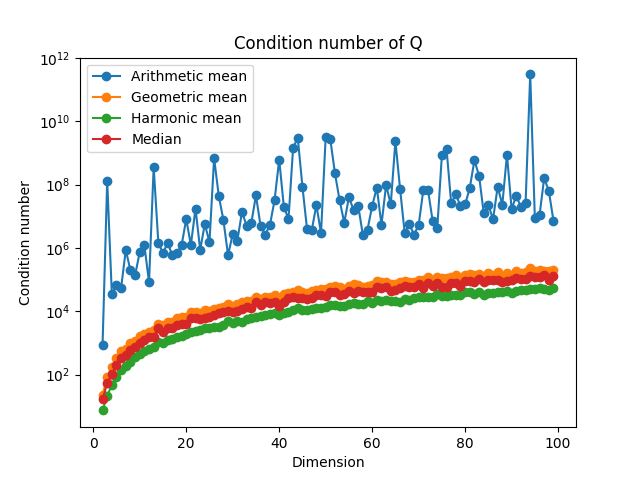
\includegraphics[width=0.8\textwidth]{part1/condition_number_vs_dims.png}
    \caption{Υπολογισμός \eng{condition number}}
\end{figure}

\clearpage
\section{Θέμα}

\clearpage
\section{Θέμα}

\clearpage
\part{Απλά Νευρωνικά Δίκτυα}
\section{Θέμα}

Παρακάτω φαίνεται κώδικας που υλοποιεί την επιθυτή έξοδο με ένα κρυφό στρώμα
νευρώνων \eng{ReLU}.

\selectlanguage{english}
\begin{python}
def relu(x):
    return max(x, 0)

# notice that the given target function can be viewed
# as follows:
def target(x):
    return abs(abs(x + 1) - 1)

def neural_network(x):
    h1 = relu(-2*x - 4)
    h2 = relu(-2*x - 2)
    h3 = relu(-x)
    h4 = relu(x)
    return relu(h1 - h2 + h3 + h4)
\end{python}
\selectlanguage{greek}

Η έξοδος του νευρωνικού δικτύου σε σχέση με την επιθυμητή έξοδο φαίνεται στο
παρακάτω διάγραμμα.

\begin{figure}[h]
    \centering
    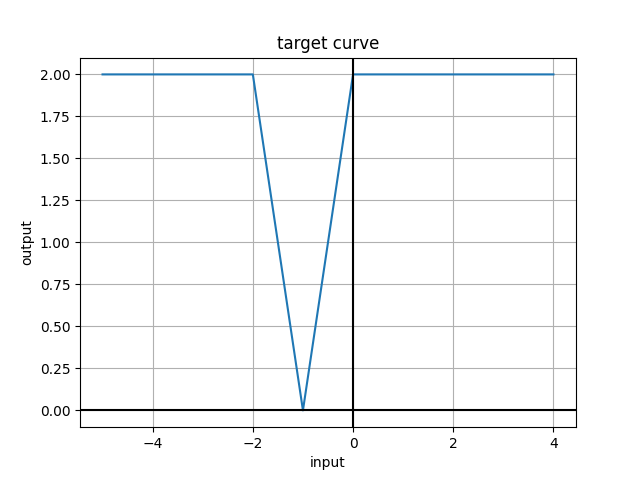
\includegraphics[width=0.8\textwidth]{part2/target-curve.png}
    \caption{Σύγκριση επιθυμητής έξοδου και εξόδου νευρωνικού δικτύου}
\end{figure}
\clearpage
\section{Θέμα}

Δεν απαντήθηκε.

\end{document}
